\documentclass[12pt,compress,aspectratio=169]{beamer}
\usetheme{metropolis}
\setbeamersize{text margin left=.5cm,text margin right=.5cm}
\usepackage[lf]{carlito}
\usepackage{siunitx}
\usepackage{tikz}
\usepackage{mathpazo}
\usepackage{bm}
\usepackage{mathtools}
\usepackage[ISO]{diffcoeff}
\diffdef{}{ op-symbol=\mathsf{d} }
\usepackage{xcolor,colortbl}

\setmonofont{Ubuntu Mono}
\setlength{\parskip}{0pt}
\renewcommand{\baselinestretch}{1}

\sisetup{
  inter-unit-product=\cdot,
  per-mode=symbol
}

\tikzset{
  >=latex
}

%\newcommand{\iii}{\hat{\bm\imath}}
%\newcommand{\jjj}{\hat{\bm\jmath}}
%\newcommand{\kkk}{\hat{\bm k}}


\setlength{\parskip}{0pt}
\renewcommand{\baselinestretch}{1}

\sisetup{
  inter-unit-product=\cdot,
  per-mode=symbol
}
\tikzset{>=latex}

\title{Topic 18: Special Relativity, Part 1}
\subtitle{AP and IBHL Physics}
\author[TML]{Dr.\ Timothy Leung}
\institute{Olympiads School}
\date{Updated: Summer 2022}

\newcommand{\pic}[2]{
  \includegraphics[width=#1\textwidth]{#2}
}
\newcommand{\eq}[2]{
  \vspace{#1}{\Large
    \begin{displaymath}
      #2
    \end{displaymath}
  }
}
%\newcommand{\iii}{\ensuremath\hat{\bm{\imath}}}
%\newcommand{\jjj}{\ensuremath\hat{\bm{\jmath}}}
%\newcommand{\kkk}{\ensuremath\hat{\bm{k}}}
\newcommand{\iii}{\ensuremath\hat\imath}
\newcommand{\jjj}{\ensuremath\hat\jmath}
\newcommand{\kkk}{\ensuremath\hat k}

\newcommand{\bigsqrt}{\ensuremath\sqrt{1-\left(\frac{v}{c}\right)^2}}
\newcommand{\lorentz}{\ensuremath\frac{1}{\bigsqrt}}



\begin{document}

\begin{frame}
  \maketitle
\end{frame}

\section{Reference Frame}

\begin{frame}{Relative Motion in Classical Physics}
  \begin{columns}
    \column{.4\textwidth}
    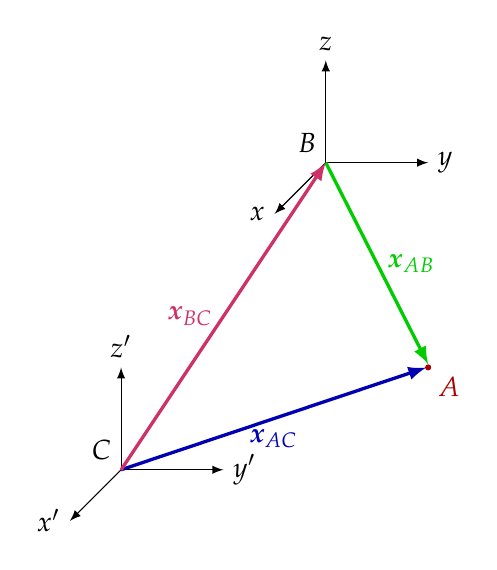
\begin{tikzpicture}[scale=1.3]
      \draw[->](0,0)--(-.5,-.5) node[left]{$x'$} node[pos=0,above left]{$C$};
      \draw[->](0,0)--(1,0) node[right]{$y'$};
      \draw[->](0,0)--(0,1) node[above]{$z'$};

      \draw[->](2,3)--(1.5,2.5) node[left]{$x$} node[pos=0,above left]{$B$};
      \draw[->](2,3)--(3,3) node[right]{$y$};
      \draw[->](2,3)--(2,4) node[above]{$z$};

      \fill[red!65!black] (3,1) circle(.03) node[below right]{$A$};
      \draw[very thick,->,blue!70!black](0,0)--(2.98,.998)
      node[midway,below]{$\bm{x}_{AC}$};
      \draw[very thick,->,green!80!black](2,3)--(3,1.03)
      node[midway,right]{$\bm{x}_{AB}$};
      \draw[very thick,->,purple!80](0,0)--(2,3)
      node[midway,left]{$\bm{x}_{BC}$};
    \end{tikzpicture}

    \column{.6\textwidth}
    In the first topic (kinematics) we studied the definitions
    \textbf{relative position}:

    \eq{-.33in}{
      \boxed{
        \textcolor{blue!70!black}{\bm{x}_{AC}}=
        \textcolor{green!80!black}{\bm{x}_{AB}}+
        \textcolor{purple!80}{\bm{x}_{BC}}
      }
    }
    
    \vspace{-.1in}\textbf{relative velocity}:

    \eq{-.25in}{
      \boxed{
        \textcolor{blue!70!black}{\bm{v}_{AC}} =
        \textcolor{green!80!black}{\bm{v}_{AB}}+
        \textcolor{purple!80}{\bm{v}_{BC}}
      }
    }

    \vspace{-.1in}and \textbf{relative acceleration}:

    \eq{-.25in}{
      \boxed{
        \textcolor{blue!70!black}{\bm{a}_{AC}}=
        \textcolor{green!80!black}{\bm{a}_{AB}}+
        \textcolor{purple!80}{\bm{a}_{BC}}
      }
    }
  \end{columns}
\end{frame}



\begin{frame}{Relative Motion}
  
  \begin{block}{}
    \textbf{All motion quantities must be measured relative to a frame of
      reference}
  \end{block}

  \vspace{.2in}
  \begin{itemize}
  \item A frame of reference is the coordinate system from which all physical
    measurements are made.
  \item Because all motions are relative, there is no absolute motion/rest
  \end{itemize}
\end{frame}  



\begin{frame}{Frame of Reference}
  Think of a \textbf{frame of reference} (or just ``frame'') as a hypothetical
  mobile ``laboratory'' an observer uses to make measurements (e.g.\ mass,
  lengths, time). At a minimum, it includes:
  \begin{itemize}
  \item Some rulers (i.e.\ coordinate system) to measure positions and lengths
  \item A clock to measure the passage of time
  \item A scale to compare forces
  \item A balance to measure masses
  \end{itemize}
\end{frame}



\begin{frame}{Frame of Reference}
  \begin{itemize}
  \item We assume that the hypothetical laboratory is \emph{perfect}---all the
    hypothetical ``instruments'' have zero errors
  \item What matters is the \emph{motion} (at rest, uniform motion, acceleration
    etc) of your laboratory, and how it affects the measurement that you make
  \item ``From the point of view of\ldots''
  \end{itemize}
\end{frame}



\begin{frame}{Inertial Frame of Reference}
  An \textbf{inertial frame of reference} (or a \textbf{rest frame}) is one
  that is moving in uniform motion
  \begin{itemize}
  \item In an inertial frame, Newton's first and second laws of motion are valid
  \item Since all uniform motion are treated the same way, you may consider
    any inertial frames of reference to be \emph{at rest}
  \end{itemize}
  \vspace{.2in}
  \begin{center}
    \fbox{
      \begin{minipage}{.8\textwidth}
        \textbf{The Principle of Relativity:} All laws of motion must apply
        equally in all inertial frames of reference.
      \end{minipage}
    }
  \end{center}
\end{frame}



\begin{frame}{Inertial Frame of Reference}
  Observer A moves uniformly with the skateboard, while Observer B stands on
  the side of the road. So, when A tosses a ball upward:
  \begin{center}
    \pic{.55}{graphics/57}
  \end{center}
  \begin{itemize}
  \item A sees only vertical motion, while
  \item B sees the ball traveling in a parabolic curve, although
  \item A \& B observe different motion, but they agree on the \emph{equations}
    that govern the motion
  \end{itemize}
\end{frame}



\begin{frame}{Inertial Frame of Reference}
  Observer A sees the same motion (only vertical motion) regardless of whether
  he is moving uniformly w.r.t.\ B or not (as long as \emph{neither} are
  accelerating)
  \begin{center}
    \pic{.55}{graphics/57.png}
  \end{center}
  \begin{itemize}
  \item Valid for A to conclude that he is at rest, but that B and the rest of
    the world are moving
  \item Likewise, it is also valid for B to think that he is at rest, but it is
    only A and his skateboard that are moving
  \end{itemize}
\end{frame}
    

\begin{frame}{Newtonian (Classical) Relativity}
  When studying kinematics and dynamics, we made some untested assumptions that
  seemed obvious: space and time are \emph{absolute}
  \begin{itemize}
  \item \SI1{\metre} is \SI1{\metre} no matter where you are, or how you are
    moving
  \item \SI1{\second} is \SI1{\second} no matter where you are, or how you are
    moving
  \item Measurements of space and time do not depend on motion
  \end{itemize}
  \vspace{.1in}If space and time are absolute, then \emph{all} velocities are
  relative to the observer
  \begin{itemize}
  \item Measured velocities depend on the motion of the observer
  \item Galilean velocity addition rule:

    \eq{-.25in}{
      \boxed{\bm{v}_{AC}=\bm{v}_{AB}+\bm{v}_{BC}}
    }
  \end{itemize}
\end{frame}


\begin{frame}{Maxwell's Equations}
  Maxwell's equations on electrodynamics in a vacuum:
  
  \vspace{-.35in}{\Large
    \begin{align*}
      \nabla\cdot\bm{E} &= 0\\
      \nabla\cdot\bm{B} &= 0\\
      \nabla\times\bm{E} &=-\frac{\partial\bm{B}}{\partial t}\\
      \nabla\times\bm{B} &=\mu_0\varepsilon_0\frac{\partial\bm{E}}{\partial t}
    \end{align*}
  }
  
  \vspace{-.1in}Disturbances in $\bm{E}$ and $\bm{B}$ travel as an
  \emph{electromagnetic wave} with a speed $c$:

  \vspace{-.25in}{\Large
    \begin{displaymath}
      c=\frac1{\sqrt{\varepsilon_0\mu_0}}=\SI{299792458}{\metre\per\second}
    \end{displaymath}
  }
\end{frame}



\begin{frame}{Peculiar features of Maxwell's equation}
  \begin{itemize}
  \item Does not mention the \emph{medium} in which EM waves travels
  \item When applying \emph{Galilean transformation} (from which we obtain
    the velocity addition rule) to Maxwell's equations, asymmetry is introduced
  \item Gauss's law for magnetism break down: magnetic field lines appear to
    have beginnings/ends
  \item In \emph{some} inertial frames of reference, Maxwell's equations are
    simple and elegant, but transform the equation into another inertial frame,
    the equations are ugly and complex!
  \item Physicists at the time began to theorize that (perhaps) there is an
    actual \emph{preferred} inertial frame of references
  \item This seems to violate the \emph{principle of relativity}
  \end{itemize}
\end{frame}



\begin{frame}{The Illusive Ether}
  Maxwell's hypothesis: the speed of light $c_0$ is relative to a hypothetical
  subtance called \textbf{luminiferous aether} (or just \textbf{ether}) that
  permeates the universe. Ether must have some fantastic properties:
  \begin{itemize}
  \item All space is filled with ether
  \item Massless
  \item Zero viscosity
  \item Non-dispersive
  \item Incompressible
  \item Continuous at a very small (sub-atomic) scale
  \end{itemize}
  It was thought that the preferred inertial reference frame is that of the
  ether
\end{frame}



\begin{frame}{Spoiler Alert}
  Spoiler alert: Ether doesn't exist.
\end{frame}



\begin{frame}{The Michelson-Morley Experiment}
  If ether exists, then at different times of the year, the Earth will have a
  different relative velocity with respect to it:
  \begin{center}
    \pic{.35}{graphics/2000px-AetherWind.png}
  \end{center}
  And it causes light to speed up or slow down. By measuring and comparing the
  speed of light at various times of the year, we should be able to determine
  to flow of ether relative to Earth.
\end{frame}



\begin{frame}{Michelson-Morley Experiment}
  American phycisists Albert Michelson\footnote{Nobel Prize in Physics, 1907}
  and Edward Morley designed an ingenious but very difficult experiment to
  detect ether using an \textbf{interferometer} designed by Michelson
  \begin{center}
    \pic{.7}{graphics/michelsonmorley.jpg}
  \end{center}
\end{frame}



\begin{frame}{The Michelson Interferometer}
  \begin{columns}
    \column{.3\textwidth}
    \begin{center}
      \pic{1.15}{graphics/313754.png}
    \end{center}

    \column{.7\textwidth}
    \begin{itemize}
    \item A beam of light is split into two using a two-way (half-silvered)
      mirror
    \item The two beams are reflected off mirrors and finally arriving at the
      screen where interference patterns are observed
    \item The two paths are the same length, so if the \emph{speed} of the light
      changes, we should see an interference pattern
    \item\textbf{Except none were ever found!} The interference patterns that
      could be observed were well within experimental errors, and far below
      expected values
    \end{itemize}
  \end{columns}
\end{frame}



\begin{frame}{What To Do with ``Null Result''}
  The Michelson-Morley experiment failed to detect the flow of ether, even
  after many refinements. What does this mean?
  \begin{itemize}
  \item Majority view
    \begin{itemize}
    \item\textbf{The experiment was flawed!} It is actually a reasonable
      guess, since the experiment is known to be a difficult one, errors can
      be introduced
    \item Keep improving the experiment (or design a better experiment) and
      Earth's motion relative to ether will eventually be found
    \end{itemize}
  \item Minority view:
    \begin{itemize}
    \item\textbf{The ether hypothesis is wrong!}
    \item The experiment showed it for what it is: ether either cannot be
      detected or it doesn't exist
    \end{itemize}
  \item A few physicists: The must be \textbf{another explanation} that saves
    both experiment and theory
  \end{itemize}
\end{frame}



\begin{frame}{Hendrik Lorentz}
  Dutch physicist Hendrik Antoon Lorentz\footnote{1853--1928, Nobel Prize in
    Physics, 1902} was one of the first to consider the findings of
  Michelson-Morley experiment to be significant
  \begin{itemize}
  \item Lorentz's hypothesis: objects traveling in the direction of ether must
    contract in length, nullifying the experimental results:

    \eq{-.2in}{
      \boxed{\beta=\bigsqrt}
    }
  \item But \emph{No known physical phenomenon} causes an object to contract
  \end{itemize}
\end{frame}



\begin{frame}{Strange Behavior in Absolute Space Time}
  French mathematician Henri Poincar\'{e} also hypothesized that ether affects
  the flow of time the direction of motion. His equation is similar to the
  hypothesis by Lorentz and contains the same factor:

  \eq{-.2in}{
    \boxed{t' =\frac{t}{\bigsqrt}}
  }
  
  But \emph{no known physical phenomenon} can alter the flow of time either!

  \uncover<2>{
    \vspace{.15in}Both Poincar\'{e} and Lorentz depended their hypothesis on
    \begin{itemize}
    \item Absolute time and space
    \item Existence of ether
    \end{itemize}
  }
\end{frame}



\begin{frame}{Making Maxwell's Equations Work}
  \begin{columns}
    \column{.2\textwidth}
    \pic{1.1}{graphics/Einstein_patentoffice.png}
    \begin{center}
      \vspace{-.15in}{\footnotesize Albert Einstein\\ in 1905\par}
    \end{center}
    
    \column{.8\textwidth}
    \begin{itemize}
    \item In 1905, at the age of 26, Albert Einstein was working as a patent
      clerk in Bern, Switzerland while completing his Ph.D.
      \begin{itemize}
      \item Believed in the principle of relativity, and therefore
      \item Rejected the concept of a ``preferred'' frame of reference
      \end{itemize}
    \item The failure of the Michelson-Morley experiment to find the flow of
      ether proves that it does not exist
    \item In order to make Maxwell's equations to work again, Einstein
      revisited two most fundamental concepts in physics: \emph{space} and
      \emph{time}
    \end{itemize}
  \end{columns}
\end{frame}


\begin{frame}{Special Relativity}
  Published in \emph{Annalen der Physik} on September 26, 1905 in the article
  \emph{On the Electrodynamics of Moving Bodies}
  \begin{itemize}
  \item Submitted on June 30, 1905 and passed for publication by a referee
  \item Einstein's third paper (of four) that year
  \item Mentions only five other scientists by name: Issac Newton, James
    Clerk Maxwell, Heinrich Hertz, Christian Doppler and Hendrik Lorentz, but
    does not contain references to any publications
  \item Ignored by most physicists at first, until Max Planck took interests
  \item Called ``special relativity'' because it describes a ``special case''
    without effects of gravity
  \end{itemize}
\end{frame}



\begin{frame}{Postulates of Special Relativity}
  \begin{center}
    \fbox{
      \begin{minipage}{.8\textwidth}
        \textbf{The Principle of Relativity:} \emph{All} laws of physics must
        apply equally in \emph{all} inertial frames of reference.
      \end{minipage}
    }
  \end{center}
  \begin{itemize}
  \item Reaffirms the principle in which physics is based on
  \item Extends the principle to include electrodynamics%(Maxwell's equations)
  \end{itemize}

  \vspace{.1in}
  \begin{center}
    \fbox{
      \begin{minipage}{.8\textwidth}
        \textbf{The Principle of Invariant Light Speed:} As measured in any
        inertial frame of reference, light always propagates in a vaccum with a
        definite velocity $c$, independent of the state of motion of the
        emitting body.
      \end{minipage}
    }
  \end{center}
  \begin{itemize}
  \item Reaffirms the results from Michelson-Morley experiment
  \item Disproves the existence of ether
  \end{itemize}
  \vspace{.1in}The two postulates are unremarkable by themselves, but when
  combined, the consequences are profound
\end{frame}



\begin{frame}{What's so Special About Special Relativity?}
  Classical (Newtonian) relativity:
  \begin{itemize}
  \item Space and time are absolute (invariant), therefore
  \item The speed of light must be relative to the observer
  \end{itemize}

  \vspace{.1in}Einstein's special relativity:
  \begin{itemize}
  \item The speed of light is absolute (invariant), therefore
  \item Space and time must be relative to the observer
  \end{itemize}

  \vspace{.1in}We must modify our traditional concepts:
  \begin{itemize}
  \item Measurement of \emph{space}
  \item Measurement of \emph{time}
  \item Concept of \emph{simultaneity}
  \end{itemize}
\end{frame}
\end{document}
